\documentclass{standalone}
\usepackage{tikz}
\usetikzlibrary{patterns, positioning}
\usepackage[sfdefault]{ClearSans} %% option 'sfdefault' activates Clear Sans as the default text font
\usepackage[T1]{fontenc}

\begin{document}
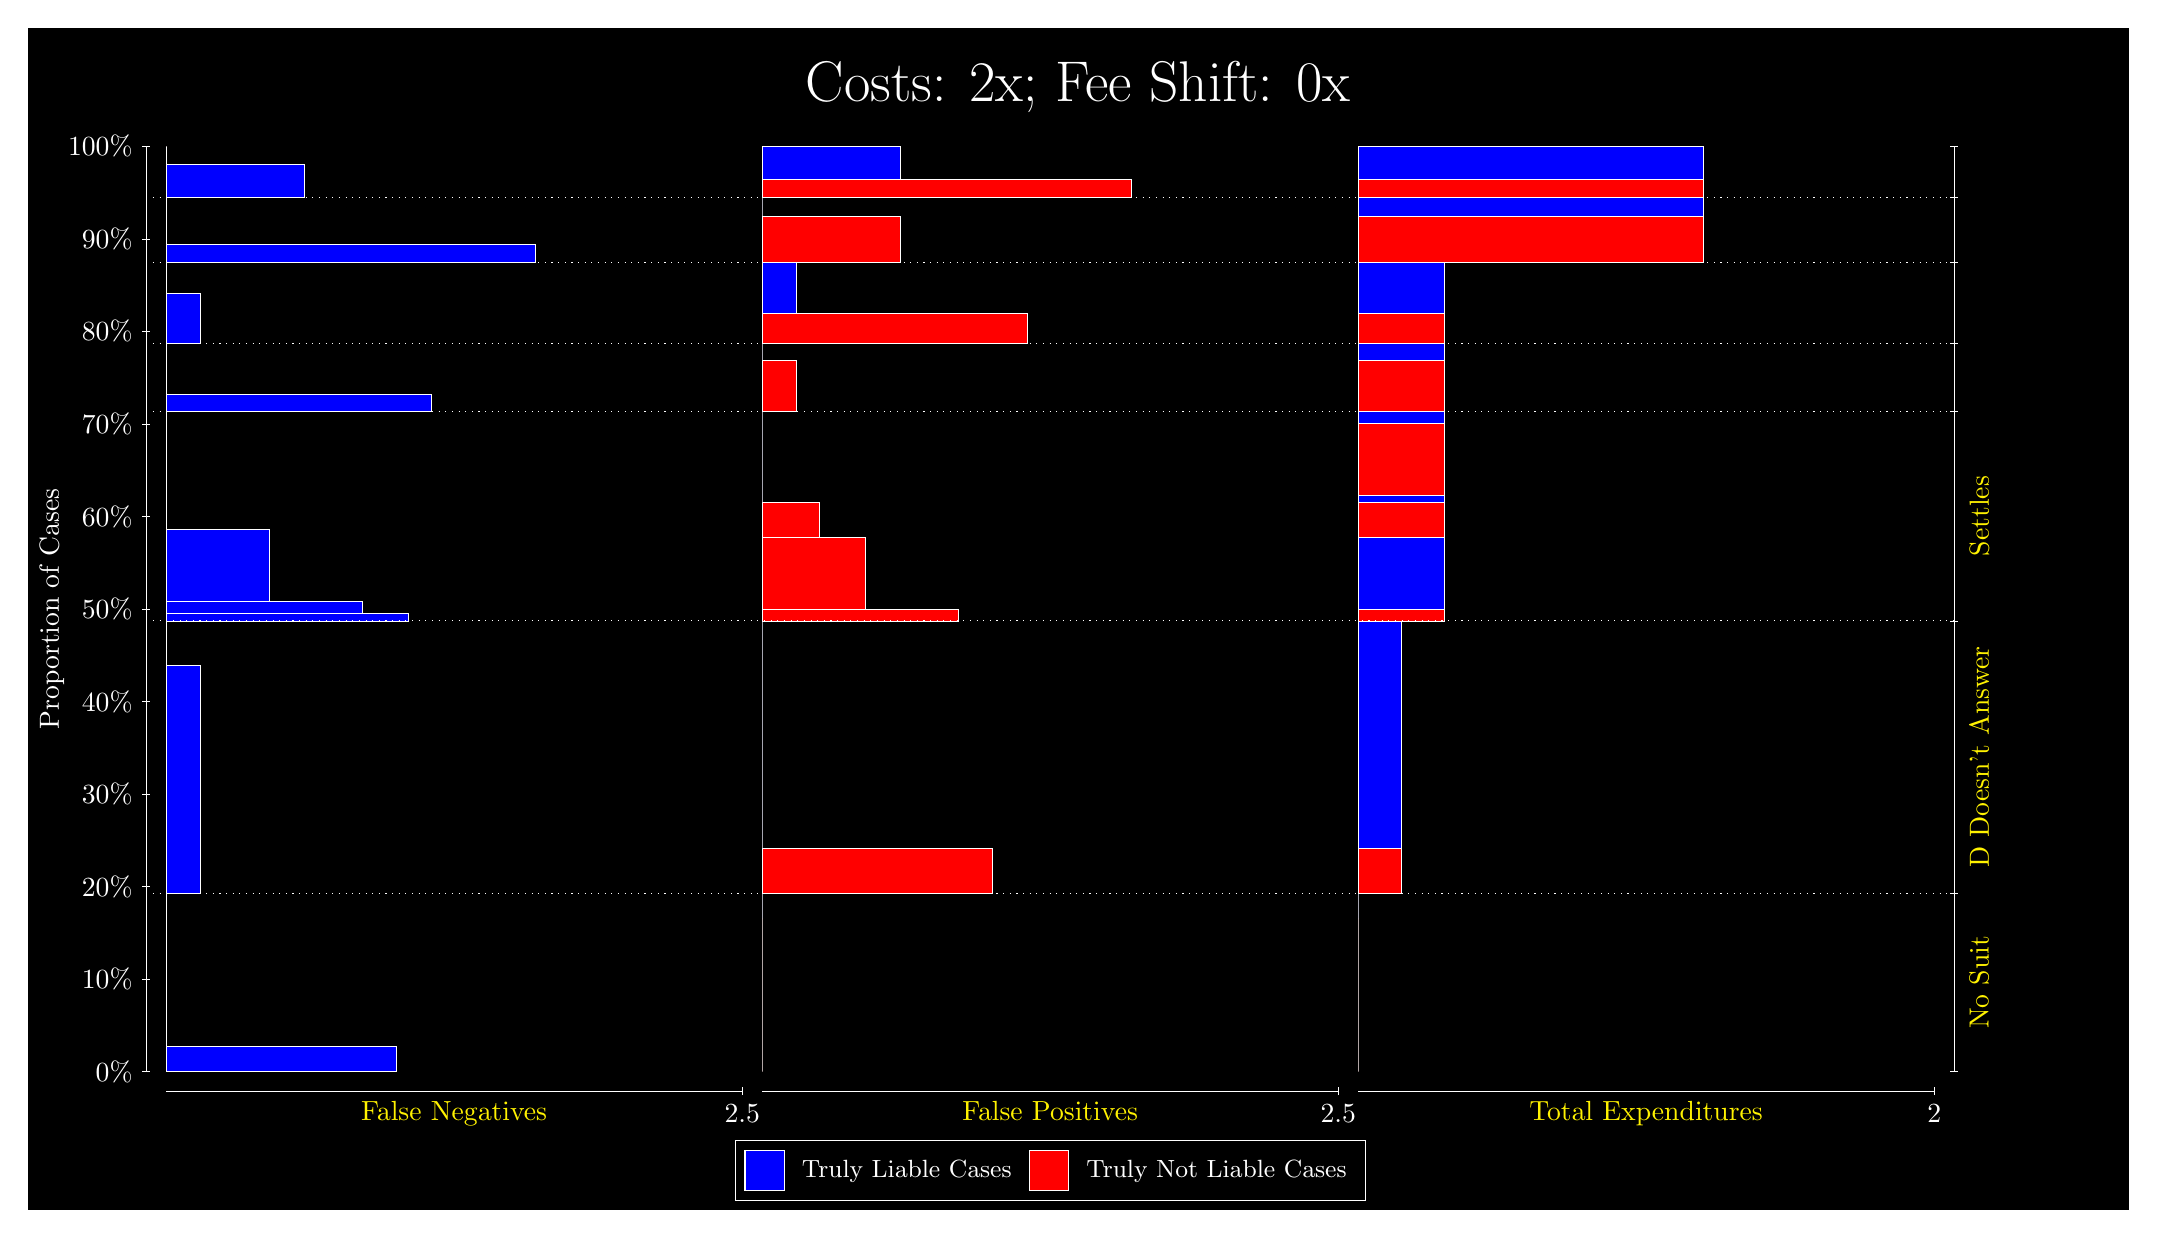
\begin{tikzpicture}
\draw[fill=black] (0,0) rectangle (26.667,15);
\draw[text=white] (0,13.5) rectangle (26.667,15) node[midway] {\huge Costs: 2x; Fee Shift: 0x};
\draw[white, very thin] (1.5,1.75) -- (1.5,13.5);
\node[rotate=90, text=white, anchor=center] at (0.3, 7.625) {Proportion of Cases};
\draw[white, very thin] (1.45,1.75) -- (1.55,1.75);
\node[text=white, anchor=east] at (1.45, 1.75) {0\%};
\draw[white, very thin] (1.45,2.925) -- (1.55,2.925);
\node[text=white, anchor=east] at (1.45, 2.925) {10\%};
\draw[white, very thin] (1.45,4.1) -- (1.55,4.1);
\node[text=white, anchor=east] at (1.45, 4.1) {20\%};
\draw[white, very thin] (1.45,5.275) -- (1.55,5.275);
\node[text=white, anchor=east] at (1.45, 5.275) {30\%};
\draw[white, very thin] (1.45,6.45) -- (1.55,6.45);
\node[text=white, anchor=east] at (1.45, 6.45) {40\%};
\draw[white, very thin] (1.45,7.625) -- (1.55,7.625);
\node[text=white, anchor=east] at (1.45, 7.625) {50\%};
\draw[white, very thin] (1.45,8.8) -- (1.55,8.8);
\node[text=white, anchor=east] at (1.45, 8.8) {60\%};
\draw[white, very thin] (1.45,9.975) -- (1.55,9.975);
\node[text=white, anchor=east] at (1.45, 9.975) {70\%};
\draw[white, very thin] (1.45,11.15) -- (1.55,11.15);
\node[text=white, anchor=east] at (1.45, 11.15) {80\%};
\draw[white, very thin] (1.45,12.325) -- (1.55,12.325);
\node[text=white, anchor=east] at (1.45, 12.325) {90\%};
\draw[white, very thin] (1.45,13.5) -- (1.55,13.5);
\node[text=white, anchor=east] at (1.45, 13.5) {100\%};

\draw[white, very thin] (24.457,1.75) -- (24.457,13.5);
\draw[white, very thin] (24.407,1.75) -- (24.507,1.75);
\node[anchor=west] at (24.407, 1.75) {};
\draw[white, very thin] (24.407,4.0136) -- (24.507,4.0136);
\node[anchor=west] at (24.407, 4.0136) {};
\draw[white, very thin] (24.407,7.474) -- (24.507,7.474);
\node[anchor=west] at (24.407, 7.474) {};
\draw[white, very thin] (24.407,10.135) -- (24.507,10.135);
\node[anchor=west] at (24.407, 10.135) {};
\draw[white, very thin] (24.407,10.997) -- (24.507,10.997);
\node[anchor=west] at (24.407, 10.997) {};
\draw[white, very thin] (24.407,12.026) -- (24.507,12.026);
\node[anchor=west] at (24.407, 12.026) {};
\draw[white, very thin] (24.407,12.847) -- (24.507,12.847);
\node[anchor=west] at (24.407, 12.847) {};
\draw[white, very thin] (24.407,13.5) -- (24.507,13.5);
\node[anchor=west] at (24.407, 13.5) {};

\draw[white, very thin, fill=blue] (1.75,1.75) rectangle (4.6775,2.0665);
\draw[white, very thin, fill=red] (1.75,2.0665) rectangle (1.75,4.0136);
\draw[white, very thin, fill=blue] (1.75,4.0136) rectangle (2.1891,6.9032);
\draw[white, very thin, fill=red] (1.75,6.9032) rectangle (1.75,7.474);
\draw[white, very thin, fill=blue] (1.75,7.474) rectangle (4.8239,7.5717);
\draw[white, very thin, fill=blue] (1.75,7.5717) rectangle (4.2384,7.7181);
\draw[white, very thin, fill=blue] (1.75,7.7181) rectangle (3.0674,8.632);
\draw[white, very thin, fill=red] (1.75,8.632) rectangle (1.75,10.135);
\draw[white, very thin, fill=blue] (1.75,10.135) rectangle (5.1167,10.352);
\draw[white, very thin, fill=red] (1.75,10.352) rectangle (1.75,10.997);
\draw[white, very thin, fill=blue] (1.75,10.997) rectangle (2.1891,11.637);
\draw[white, very thin, fill=red] (1.75,11.637) rectangle (1.75,12.026);
\draw[white, very thin, fill=blue] (1.75,12.026) rectangle (6.4341,12.256);
\draw[white, very thin, fill=red] (1.75,12.256) rectangle (1.75,12.847);
\draw[white, very thin, fill=blue] (1.75,12.847) rectangle (3.5065,13.271);
\draw[white, very thin, fill=red] (1.75,13.271) rectangle (1.75,13.5);
\draw[white, very thin, fill=red] (9.3189,1.75) rectangle (9.3189,3.6972);
\draw[white, very thin, fill=blue] (9.3189,3.6972) rectangle (9.3189,4.0136);
\draw[white, very thin, fill=red] (9.3189,4.0136) rectangle (12.246,4.5845);
\draw[white, very thin, fill=blue] (9.3189,4.5845) rectangle (9.3189,7.474);
\draw[white, very thin, fill=red] (9.3189,7.474) rectangle (11.807,7.6204);
\draw[white, very thin, fill=red] (9.3189,7.6204) rectangle (10.636,8.5343);
\draw[white, very thin, fill=red] (9.3189,8.5343) rectangle (10.051,8.9767);
\draw[white, very thin, fill=blue] (9.3189,8.9767) rectangle (9.3189,10.135);
\draw[white, very thin, fill=red] (9.3189,10.135) rectangle (9.758,10.78);
\draw[white, very thin, fill=blue] (9.3189,10.78) rectangle (9.3189,10.997);
\draw[white, very thin, fill=red] (9.3189,10.997) rectangle (12.686,11.386);
\draw[white, very thin, fill=blue] (9.3189,11.386) rectangle (9.758,12.026);
\draw[white, very thin, fill=red] (9.3189,12.026) rectangle (11.075,12.617);
\draw[white, very thin, fill=blue] (9.3189,12.617) rectangle (9.3189,12.847);
\draw[white, very thin, fill=red] (9.3189,12.847) rectangle (14.003,13.076);
\draw[white, very thin, fill=blue] (9.3189,13.076) rectangle (11.075,13.5);
\draw[white, very thin, fill=red] (16.888,1.75) rectangle (16.888,3.6972);
\draw[white, very thin, fill=blue] (16.888,3.6972) rectangle (16.888,4.0136);
\draw[white, very thin, fill=red] (16.888,4.0136) rectangle (17.437,4.5845);
\draw[white, very thin, fill=blue] (16.888,4.5845) rectangle (17.437,7.474);
\draw[white, very thin, fill=red] (16.888,7.474) rectangle (17.986,7.6204);
\draw[white, very thin, fill=blue] (16.888,7.6204) rectangle (17.986,8.5342);
\draw[white, very thin, fill=red] (16.888,8.5342) rectangle (17.986,8.9767);
\draw[white, very thin, fill=blue] (16.888,8.9767) rectangle (17.986,9.0744);
\draw[white, very thin, fill=red] (16.888,9.0744) rectangle (17.986,9.9883);
\draw[white, very thin, fill=blue] (16.888,9.9883) rectangle (17.986,10.135);
\draw[white, very thin, fill=red] (16.888,10.135) rectangle (17.986,10.78);
\draw[white, very thin, fill=blue] (16.888,10.78) rectangle (17.986,10.997);
\draw[white, very thin, fill=red] (16.888,10.997) rectangle (17.986,11.386);
\draw[white, very thin, fill=blue] (16.888,11.386) rectangle (17.986,12.026);
\draw[white, very thin, fill=red] (16.888,12.026) rectangle (21.279,12.617);
\draw[white, very thin, fill=blue] (16.888,12.617) rectangle (21.279,12.847);
\draw[white, very thin, fill=red] (16.888,12.847) rectangle (21.279,13.076);
\draw[white, very thin, fill=blue] (16.888,13.076) rectangle (21.279,13.5);
\draw[white, dotted] (1.5,4.0136) -- (24.457,4.0136);
\draw[white, dotted] (1.5,7.474) -- (24.457,7.474);
\draw[white, dotted] (1.5,10.135) -- (24.457,10.135);
\draw[white, dotted] (1.5,10.997) -- (24.457,10.997);
\draw[white, dotted] (1.5,12.026) -- (24.457,12.026);
\draw[white, dotted] (1.5,12.847) -- (24.457,12.847);
\draw[white, very thin] (1.75,1.5) -- (9.0689,1.5);
\node[text=yellow, anchor=north] at (5.4094, 1.5) {False Negatives};
\draw[white, very thin] (9.0689,1.45) -- (9.0689,1.55);
\node[text=white, anchor=north] at (9.0689, 1.45) {2.5};

\draw[white, very thin] (9.3189,1.5) -- (16.638,1.5);
\node[text=yellow, anchor=north] at (12.978, 1.5) {False Positives};
\draw[white, very thin] (16.638,1.45) -- (16.638,1.55);
\node[text=white, anchor=north] at (16.638, 1.45) {2.5};

\draw[white, very thin] (16.888,1.5) -- (24.207,1.5);
\node[text=yellow, anchor=north] at (20.547, 1.5) {Total Expenditures};
\draw[white, very thin] (24.207,1.45) -- (24.207,1.55);
\node[text=white, anchor=north] at (24.207, 1.45) {2};

\node[text=yellow, centered, rotate=90] at (24.777, 2.8818) {No Suit};
\node[text=yellow, centered, rotate=90] at (24.777, 5.7438) {D Doesn't Answer};
\node[text=yellow, centered, rotate=90] at (24.777, 8.8043) {Settles};





\draw (12.978300999999998,1.5) node[draw=none] (baseCoordinate) {};
\begin{scope}[align=center]
        \matrix[scale=0.5, draw=white, below=0.5cm of baseCoordinate, nodes={draw}, column sep=0.1cm]{
            \node[rectangle, draw, minimum width=0.5cm, minimum height=0.5cm, fill=blue] {}; &
            \node[draw=none, font=\small, text=white] (B) {Truly Liable Cases}; &
            \node[rectangle, draw, minimum width=0.5cm, minimum height=0.5cm, fill=red] {}; &
            \node[draw=none, font=\small, text=white] (B) {Truly Not Liable Cases}; \\
            };
\end{scope}

\end{tikzpicture}
\end{document}